\documentclass[12pt]{article}
\usepackage[margin=1.2in]{geometry}
\usepackage{float,graphicx}
\usepackage{enumitem}
\usepackage{listings}
\usepackage{hyperref}

\title{C S 378: Concurrency: Thread Pools for I/O Bound Processes}
\author{
        Allen Jue \\
        Department of Computer Science\\
        UT Austin
}\date{\today}

\begin{document}

\maketitle

\section{Abstract}

Thread pools are collections of threads that perform asynchronous callbacks and help reduce overhead associated with creating and managing large numbers of threads for unpredictable workloads. Satisfying network requests is an ideal workload for a thread pool, as requests from clients over a network can be unreliable and unpredictable. Moreover, the tasks are I/O bound, so the asynchronous nature of thread pools can avoid excess waiting. This project explores Boost C++'s thread pool and implements its own version of a thread pool that creates a callable object with C/C++'s \texttt{std::bind}. The results were measured by comparing the speedup of the two thread pools to the sequential implementation and measuring the increase in number of requests dropped. The Boost thread pool implementation experienced up to a 1.75x execution time speedup and my personal thread pool implementations experienced up to 1.86x execution time speedup for multi-threaded approaches for thread pools through a size of 16 threads. For both thread pool implementations, there were significant accuracy penalties up to 82.2\% for thread pools exceeding a size of 16 threads. Overall, by observing the trade-offs between accuracy and speedup, utilizing a thread pool for I/O bound requests can provide a significant performance benefit.

\section{Introduction}

Thread pools are a programming design pattern, where a number of threads are created in reserve to service multiple tasks dynamically. The tasks can be independent or have some form of communication. Regardless, the purpose of this design pattern is to reduce the significant time required to spin up and deconstruct a thread. This design pattern can be seen in web servers, where worker threads spawned within a thread pool can wait for tasks to intermittently come in, and the size of the thread pool can be dynamically adjusted to suit changing workloads. It should be noted that the number of threads in a thread pool is a parameter that needs to be carefully tuned, as having too many threads idly waiting is also an inefficient use of resources.

For this project, I compiled a list of the 42 most visited websites in the world. I figured that these websites would be trustworthy and reliable to try and confirm basic network connectivity. I then created a method that would call \texttt{popen(("ping -c 1 -t 1 " + website, "r");}. This creates a readable pipe from the command that I provided it, which would allow me to:
\begin{enumerate}
    \item Ping the specified website \textbf{once}
    \item Time out after 1 second
    \item Read the results into a buffer 
    \item Determine if any packets were lost
\end{enumerate}

Now that I had a reusable method that could ping a list of websites, I just needed to create thread pools, from which I could submit tasks that would call my custom   \texttt{popen()} method and measure the changes in execution time and accuracy as I tuned the number of threads within a thread pool. On the testing machine, I ran 
\texttt{std::thread::hardware\_concurrency}, which returns the number of threads supported on my machine. In this case, it was 16, so I would expect limited returns from thread pools over a size of 16.

\section{Implementations}

\subsection{Sequential}

The sequential implementation calls the \texttt{popen()} method for each website. The sequential implementation provides a baseline for the execution time, with an average runtime of 3.461231200 and 0 errors when run 10 times to reduce variance.

\subsection{Boost ASIO}

The boost library implementation creates a thread pool with the number of threads specified by the command line argument with \texttt{boost::asio::thread\_pool}. Then, for each website, a lambda function is created that captures the the current website and index by reference and invokes the \texttt{popen()} method to make a ping request and stores the result in a vector of results. Finally, there is a \texttt{pool.join()} call that blocks until each worker thread is done, closing the thread pool and preventing any more incoming requests. 

\subsection{Personal Implementation}

To create a thread pool, I first needed to implement a thread-safe bounded buffer. The bounded buffer enables multiple threads to safely enqueue and poll objects. When the bounded buffer decides to refuse further work, it can be explicitly closed with a \texttt{closeBuffer()} method.

The \texttt{ThreadPool} class utilizes a bounded buffer as its underlying data structure to store work that can be submitted dynamically. It also has a vector of worker threads that are kept as a reference to be deconstructed when the thread pool is closed. When work is submitted to the thread pool, it is submitted in the form of \texttt{submit(F f, Args\&\&... args)}. Worker threads busy-wait in a while loop for work until the thread pool is closed. The first parameter represents the function and the Args is a list of references to the arguments. With this, I was able to use \texttt{std::bind} and \texttt{std::forward} to forward the arguments as an rvalue and generate a new function with the arguments bound to the method. When the thread pool is closed, it joins each worker, refusing more work and blocking until all workers have been collected. 

Overall, my thread pool implementation was based heavily on the Boost ASIO libraries implementation, as I wanted to create similar methods and constructors.
\begin{enumerate}
    \item Constructors
    \begin{enumerate}
        \item boost::asio::thread\_pool pool(std::size\_t num\_threads); 
        \item ThreadPool::ThreadPool(int threads) 
    \end{enumerate}
    \item Submiting work
    \begin{enumerate}
        \item   void post(BOOST\_ASIO\_MOVE\_ARG(Function) f, const Allocator\& a) const;
        \item void submit(F f, Args\&\&... args)
    \end{enumerate}
    \item Closing Thread Pool
    \begin{enumerate}
        \item   BOOST\_ASIO\_DECL void join();
        \item   void ThreadPool::close()
    \end{enumerate}
\end{enumerate}
I found the Boost ASIO implementation simple to use. While Boost ASIO supports futures, my implementation makes a simplifying assumption that the method passed in is a void method, limiting its flexibility and requiring the user to make an effort to store a reference to the return value somewhere if that is the desired behavior.


\section{Results}

To capture the results in a reliable way, I recorded the timings on the same network consecutively. To account for variability, I averaged the execution time and number of dropped packets for a variable number of threads 10 times. 

\subsection{Speedup}
    The sequential implementation took 3.461231200 seconds, and the results show that both thread pool implementations performed optimally with 2 threads. The performance stays better than the sequential implementation until 16 threads, at which point, my personal implementation becomes about the same as the sequential. The Boost ASIO implementation only becomes worse at 32 threads. 

    \begin{figure}[H]
        \centering
        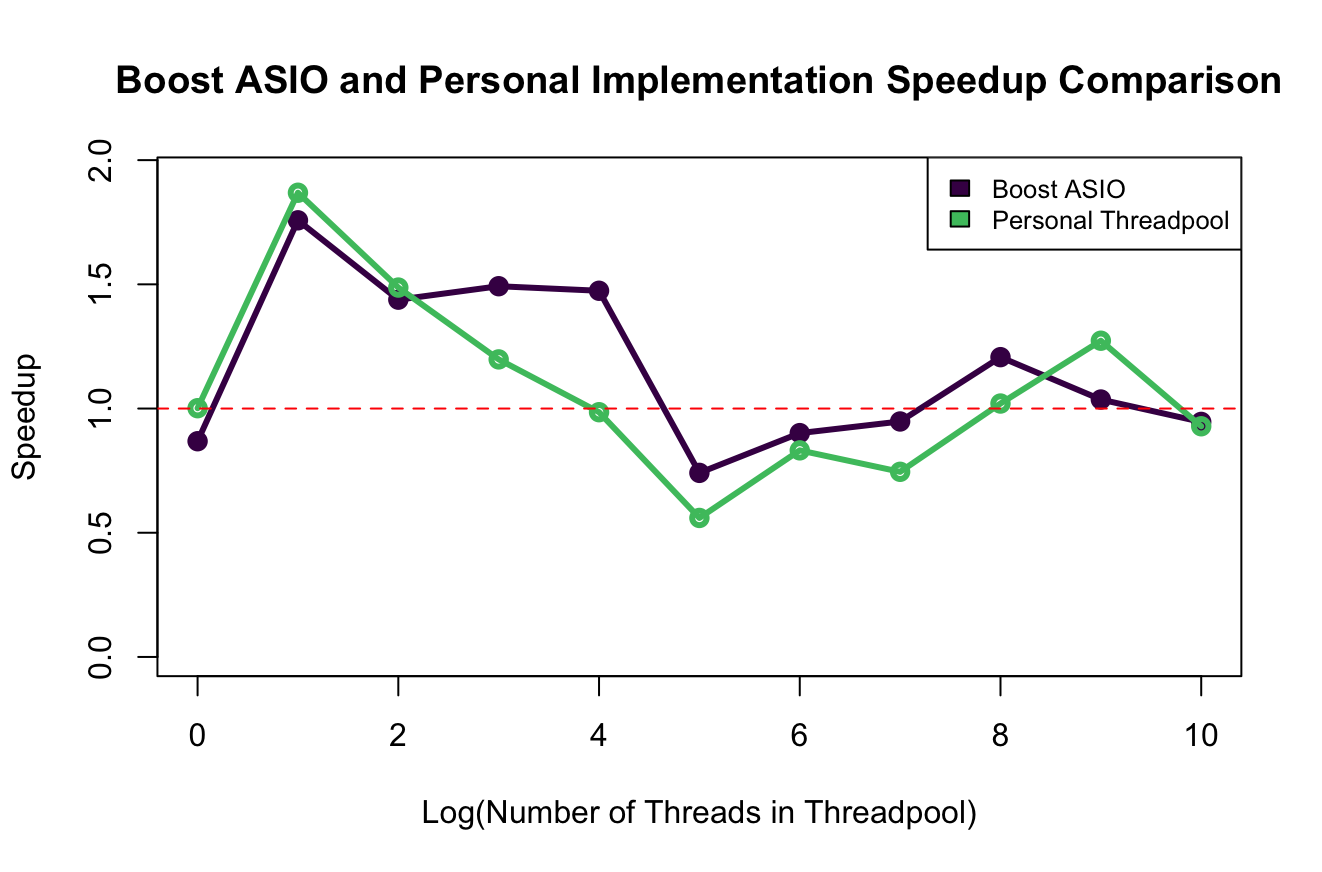
\includegraphics[width = 1.0\linewidth]{speedupComp.png}
        \caption{Personal implementation reaches max speedup of: 1.868739 x and the Boost ASIO implementation reaches max speedup of: 1.75773 x.}
    \end{figure}

    The 16 thread boundary for performance makes sense, as the hardware can only support true concurrency of up to 16 threads. Any more threads would put higher strain on the processors. Moreover, since there are not that many requests to satisfy, I imagine that beyond 16 threads, there may be significant busy waiting that negatively affects the speedup. 

    Another interesting result is that my thread pool at its best performs better than the Boost ASIO library thread pool. It's possible that this is due to network variability. Another reason is that with a smaller workload, non-blocking thread pools may perform better. Boost ASIO has something called an IO\_context, which notifies workers when work has been submitted. This is better for unpredictable and larger workloads, as CPU cycles aren't burnt uselessly. This has a consequence of being slower for smaller workloads, as busy-waiting with low contention may use less instructions than blocking a worker thread. As the number of threads increases, since my implementation implements busy waiting for work, there is more contention and wasted cycles, so its performance decreases more dramatically. 

    As the number of threads increases significantly (beyond 128 threads), both implementations exhibit an improving execution time. This is misleading, as the accuracy for these sizes of thread pools is extremely poor. Almost everything fails, and the execution time improves due to timeouts for each thread. 
\subsection{Accuracy}
    
   The accuracy for both thread pool implementations increases exponentially after the number of threads exceeds 16. It should be noted that any performance benefit enjoyed after a thread pool of size 16 is nearly useless, as it contains as much as 82.2\% failed requests. Fortunately, for thread pools with sizes not exceeding 16, there are essentially 0 dropped packets.

   
    \begin{figure}[H]
        \centering
        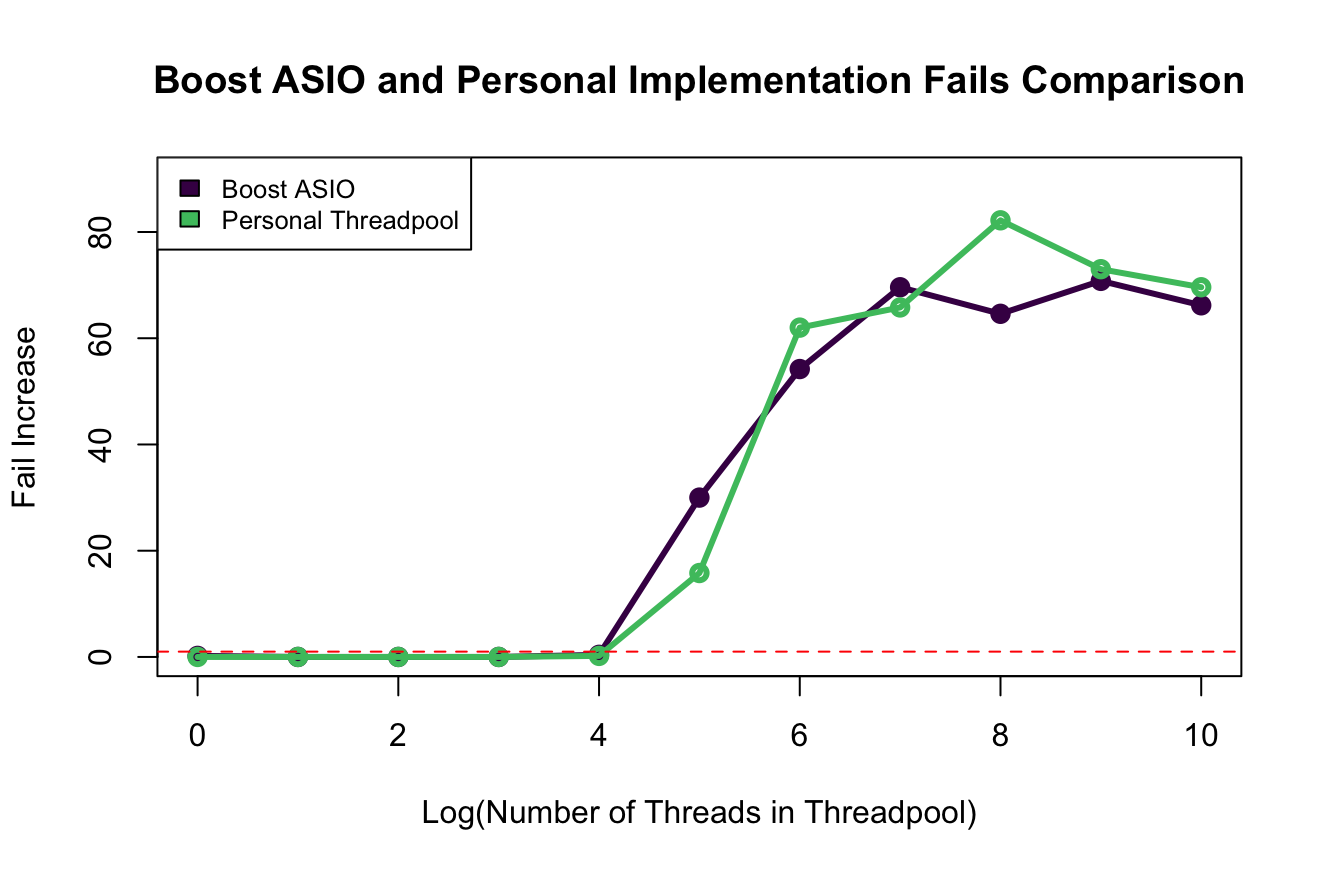
\includegraphics[width = 1.0\linewidth]{failComp.png}
        \caption{There is a dramatic increase in errors beyond thread pools of size 16.}
    \end{figure}

   As mentioned before, the improvement in run time can be seen in two areas: when failed messages are essentially obsolete and when failed messages are the majority. There are a few explanations for this behavior:
    \begin{enumerate}
        \item Resource exhaustion - there are a limited number of file descriptors and network sockets. Creating too many at once may overwhelm the system
        \item Network limitations - the network may be overwhelmed with trying to satisfy too many requests
        \item Timeout limitations - since the timeout is set to 1 second, the request may start, but many threads may run in between, causing it to timeout by default
    \end{enumerate}

    It is almost never acceptable to have this high of a failure rate. Even with the slight performance benefit, it would be prudent to maintain a thread pool with a size at most the number of threads the hardware limits.
    
\section{Summary}

Thread pools are an extremely powerful tool to manage resources and maintain the parallel benefits of utilizing threads. In the case of I/O bound tasks, threads can shine due to the asynchronous nature of sending requests and receiving their results. In this lab, I implemented a thread pool that exceeded the peak performance of Boost ASIO's thread pool. Moreover, it was observed that attempting to create thread pools beyond the size of the machine's limits would dramatically affect the accuracy of the results and provide erroneous performance benefits. Overall, it should be remembered that when working with a thread pool, it is extremely beneficial to observe the empirical benefit or detriments of different thread pool sizes and tune that parameter accordingly.

\end{document}
